\documentclass[onecolumn,12pt]{asme2ej}
\usepackage{epsfig}\usepackage{amsmath}\usepackage{amsfonts}
\usepackage{amssymb}\usepackage{graphicx}\pagenumbering{arabic}
\usepackage{verbatim}\usepackage[utf8]{inputenc}\usepackage[portuguese]{babel}
\providecommand{\keywords}[1]{\small\textbf{\textit{Keywords---}} #1}
\usepackage{comment}
\usepackage[backend=biber,style=numeric,sorting=none]{biblatex}
\usepackage{fancyhdr}\usepackage{pifont}
\usepackage{tikzsymbols}\usepackage{placeins}
\usepackage{rotating}
\pagestyle{fancy}\fancyhf{}\rfoot{Página \thepage}

\addbibresource{mybib.bib} \iffalse É neste arquivo que as referências ficam. \fi

\title{ Relatório sobre uso de GANs para o aumento de imagens de glóbulos vermelhos no conjunto de dados }

\author{Eduardo Eiji Goto \affiliation{PUCPR\\Ciência da Computação\\eduardo.goto@pucpr.edu.br}}

\author{Gustavo Hammerschmidt\affiliation{PUCPR\\Ciência da Computação\\g.hammerschmidt@pucpr.edu.br}}

\author{João Vitor Andrioli \affiliation{PUCPR\\Ciência da Computação\\joao.vitor.andrioli@gmail.com}}

\begin{document}

\maketitle 

$\\ \\ \\$

{\it 

    Neste relatório descrevemos os processos que os autores: Oleksandr Bailo, DongShik Ham, e Young Min Shin Noul Inc utilizaram para aplicar as técnicas de tradução de imagem a imagem em lâminas de extensão sanguínea {\it (blood smears)} para aumentar significativamente pequenos conjuntos de dados. A partir das máscaras de segmentação das imagens obtidas com microscópios, eles foram capazes de gerar imagens foto-realistas de glóbulos vermelhos, utilizadas juntas aos dados reais durante o treinamento da rede para tarefas de segmentar e detectar objetos. O método usado é baseado em redes adversárias generativas condicionais, pois suas capacidades comprovam uma síntese de imagens com alta-qualidade. Fora sintetizar as imagens de sangue, os autores sintetizaram as máscaras de segmentação também, o que levou a uma variedade maior nas amostras geradas. A efetividade da técnica foi contrastada com as análises de muitos experimentos coletados manualmente.
    
}

\newpage \tableofcontents \newpage


\section{Descrição do Problema}

A aquisição de conjuntos de dados médicos para tarefas de Aprendizagem de Máquina passa por muitas dificuldades. Primeiramente, o pré-processamento dos dados precisa ser feito por um especialista da área. Descritores comuns, como rótulos e máscaras de segmentação, não podem ser facilmente aplicados tanto por motivos técnicos quanto éticos. Além disso, a quantidade de dados disponíveis não é suficiente para se montar um conjunto de dados considerável, sendo necessário que haja uma junção dos dados gerados por diversas instituições (o que gera ainda mais burocracia). Por fim, diferenças de protocolos de amostras médicas entre países impedem que haja uma padronização dos dados.

De acordo com os autores do artigo (Bailo, O; Ham, D; e Noul, Y), o trabalho \cite{redblood} tem como objetivo explorar a possibilidade de se usar Redes Adversárias Generativas (GANs) como método de Augmentação (aumentar a quantidade de dados disponíveis) para as tarefas de Segmentação e detecção de objetos. Mais especificamente, utiliza-se GANs, junto a Máscaras de Segmentação sintéticas para gerar amostras sintéticas foto-realísticas de Lâminas de Extensão Sanguínea {\it (blood smears)}. A figura 1 apresenta o pipeline das tarefas de forma simplificada, além de indicar em que momento do mesmo faz-se uso de uma Rede Adversária Generativa.

\FloatBarrier
\begin{figure}[h]
    \centering
    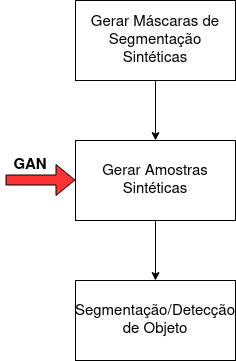
\includegraphics[width=5cm]{gansPics/fluxo.png}
    \caption{Fluxo do projeto. Fonte: Oleksandr, B; Ham, D; e Noul, Y.}
    \label{fig:fig1}
\end{figure}
\FloatBarrier

Em um primeiro momento, são geradas máscaras sintéticas. Essas máscaras são geradas automaticamente e serão utilizadas como input para a GAN em questão. O formato e distribuição dos glóbulos na máscara são definidos a partir de um conjunto de dados de exemplos de células. Utiliza-se um pequeno conjunto de dados de lâminas tanto para popular o conjunto de exemplos de células quanto para treinar a GAN. O objetivo é gerar uma quantidade considerável de dados sintéticos a partir de uma quantidade limitada de dados reais. A figura 2 ilustra o resultado final da rede generativa, a primeira linha é composta pela máscara e imagem de um exemplo real, por outro lado, a segunda linha representa uma máscara sintética e a imagem gerada a partir desta máscara.

\FloatBarrier
\begin{figure}[h]
    \centering
    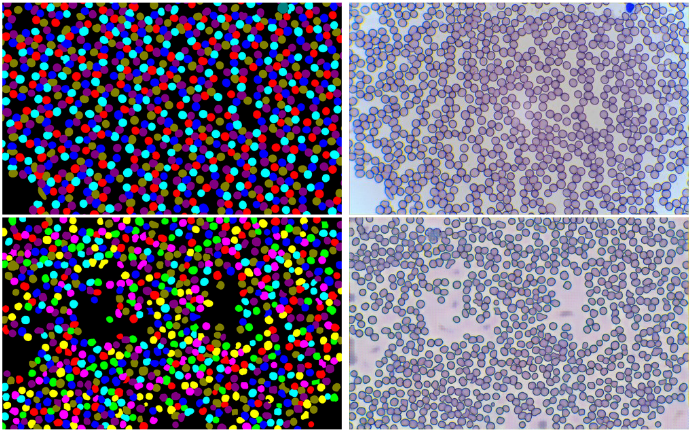
\includegraphics[width=14cm]{gansPics/examples_intro.png}
    \caption{Exemplo dos resultados da GAN. Fonte: Oleksandr, B; Ham, D; e Noul, Y.}
    \label{fig:fig2}
\end{figure}
\FloatBarrier

Os autores aplicam, então, o uso de técnicas de tradução de imagem para imagem para usar as lâminas sanguíneas e, a partir delas, conseguir novas amostras de dados e aumentar significativamente o tamanho dos conjuntos de dados com essa técnica. O uso de GANs prove uma síntese de alta-qualidade dessas imagens, o que é viável para gerar dados sintéticos condizentes com dados reais e foto-realísticos. A coleta das 100 imagens com distinções consideráveis entre si serve características relevantes ao modelo que, portanto, deriva delas um mapa de distribuição dos glóbulos.


\section{Base}

O conjunto de dados utilizado de glóbulos vermelhos foi obtido a partir da coleta de sangue de 100 pacientes, o sangue foi preparado e as imagens coletadas utilizando um "microscópio de campo claro" que busca aumentar o contraste entre a amostra escura e o fundo claro, ou vice-versa, as imagens possuem 40x de magnitude.

Como a tarefa é a geração de imagens, o conjunto de dados não possui desbalanceamento de classes, pois não possui classes, mas possui a variação na distribuição dos glóbulos vermelhos que possuem cores, formatos e quantidades diferentes em cada imagem. Para garantir distribuições significantes e a diversidade das imagens, foram selecionadas manualmente 100 imagens com características distintas.

Os autores utilizaram uma técnica de processamento das imagens para melhorar a separação dos glóbulos, que consiste em colorir manualmente cada glóbulo de uma cor diferente, de forma que seja mais fácil para o algoritmo identificar cada glóbulo sem ocorrer a sobreposição de vários.

As imagens possuem 1920x1200 de resolução no formato RGB e os autores utilizam 60 imagens para treino e 40 imagens para teste, ver figura 3.

\FloatBarrier
\begin{figure}[h]
    \centering
    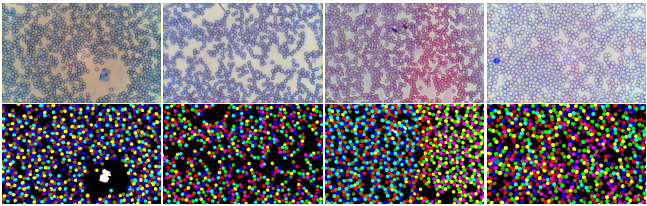
\includegraphics[width=14cm]{gansPics/dataset.png}
    \caption{Amostras do conjunto de dados. Fonte: Oleksandr, B; Ham, D; e Noul, Y.}
    \label{fig:fig3}
\end{figure}
\FloatBarrier

A imagem a seguir demonstra o motivo dos autores preferirem o uso de GANs nessa tarefa. Afinal, a diversidade das imagens está expressa por uma função de distribuição identitária, e o uso de algoritmos de geração aleatória acabariam por distribuir aleatoriamente em porções quase que equivalentes - ignorando um fenômeno importante para a medicina que seria o acúmulo de células em certas regiões, pois podem expressar uma região de criação de células, ou uma região onde há gordura sendo armazenada, ou até mesmo alguma mutação local.

\FloatBarrier
\begin{figure}[h]
    \centering
    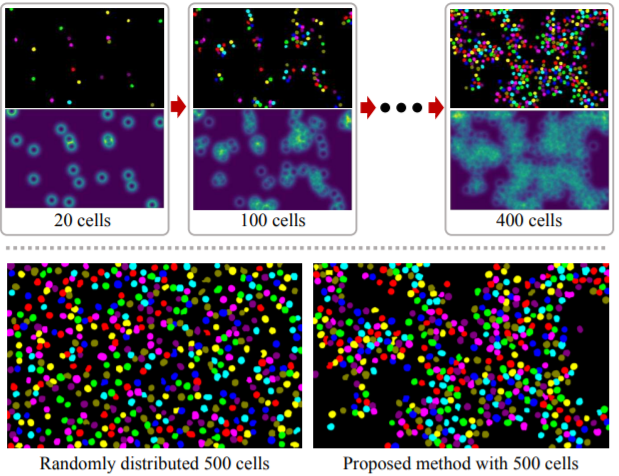
\includegraphics[width=14cm]{gansPics/fig4.PNG}
    \caption{Geração de máscara sintética. (Acima) compara a segmentação e um mapa possível para o algoritmo, (Abaixo) compara o resultado de distribuição aleatória e a distribuição com o método proposto. Fonte: Oleksandr, B; Ham, D; e Noul, Y.}
    \label{fig:fig4}
\end{figure}
\FloatBarrier


\section{Arquitetura de Rede/Solução}

A metodologia usada divide a criação de novas amostras em duas etapas: geração de máscaras sintéticas e tradução das máscaras geradas para imagens foto-realistas de glóbulos vermelhos. A imagem abaixo mostra todo o processo do modelo durante o seu treino e teste.  

\FloatBarrier
\begin{figure}[h]
    \centering
    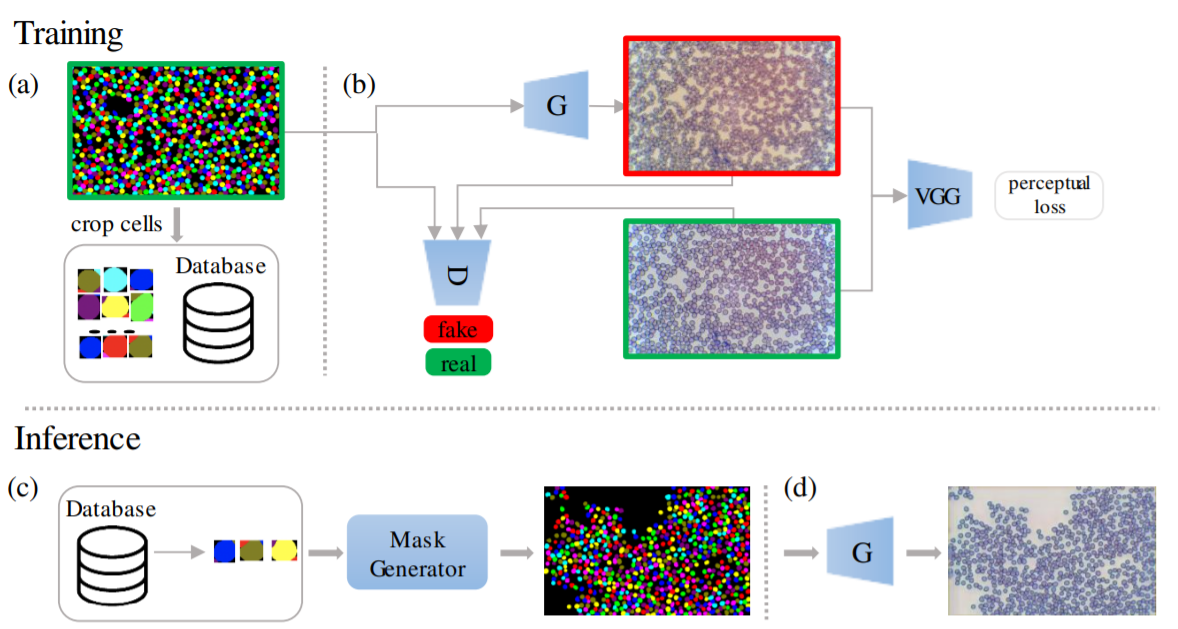
\includegraphics[width=14cm]{gansPics/fig5.PNG}
    \caption{Método proposto. Fonte: Oleksandr, B; Ham, D; e Noul, Y.}
    \label{fig:fig5}
\end{figure}
\FloatBarrier

As instâncias da forma dos glóbulos são extraídas e salvas no banco de dados (a). Durante isso, o {\it framework} pix2pixHD (um modelo proposto por Wang et al - ele produz imagens de alta-resolução foto-realistas a partir de instâncias de máscaras de segmentação de uma cena; ele permite uma fácil manipulação interativa dos objetos na cena, levando a muitas novas amostras) é treinado para traduzir máscaras de segmentação para imagens de glóbulos (b). Durante o estágio de inferência, máscaras de segmentação sintéticas são geradas (c) e utilizadas para carregar a rede do gerador ({\it generator}) para que ele produza as imagens realistas dos glóbulos (d).

Para que a amostra gerada seja significativa para o conjunto de dados e foto-realista, as instâncias sintéticas de máscaras de segmentação produzidas devem ter as características das imagens usadas como input: formas únicas e a forma com a qual a sua distribuição ocorre ({\it location distribution}); logo, os autores desenvolveram um {\it generator} de máscaras de segmentação sintética com o propósito de combinar as duas características.

Para isso, eles formularem um conjunto matemático que explicita o par de valores: formato do glóbulo e localização correspondente na imagem de fundo. O número de glóbulos em uma imagem é derivado a partir da distribuição normal, onde a média e o desvio padrão usado na equação são derivados das estatísticas do conjunto de dados de treino.

Com relação ao formato do glóbulo, o processo de obtenção de novas instâncias se dá por amostragem de glóbulo baseada em exemplos a partir dos conjuntos de dados de treino e de teste.

Na fase de treino, os limites segmentados de cada glóbulo no conjunto de dados de treino são acumulados para construir um banco de dados de formatos de células. Então, eles são convertidos para uma representação em binário e armazenados como uma lista de imagens. E esse banco de dados é usado no estágio de inferência (c) para que, durante esse processo, os formatos sejam selecionados aleatoriamente e colocados na máscara de segmentação - uma máscara possui várias células. A cada chamada a base, um conjunto de augmentações probabilísticas (segundo os autores) são aplicadas às imagens para diversificar a aparência e, com isso então, gerar imagens não-vistas de células. O processo de augmentação inclui rotação, {\it scale} (escala, proporção), e inversões da imagem no eixo horizontal e vertical.

Devido a propriedade de adesão das células entre si, usar uma distribuição que ocupe lugares vazios em uma imagem resulta em uma imagem irreal, pois elas tendem a formar clusters. Portanto, o algoritmo utiliza uma distribuição de amostras sequencialmente de forma coerente com a função de densidade probabilística definida. Para isso, eles modelarem esse fenômeno como sendo um processo aleatório de Markov.

Na prática, uma cor específica é atribuída a cada célula colocada na imagem, satisfazendo a condição de que nenhuma célula que tocando outra tenha a mesma cor. Se essa condição for falsa, é usado um novo mapa com coordenadas novas para as amostras de células de forma que elas satisfaçam a condição imposta. Então, todas as máscaras sintéticas produzidas podem ser tratadas como as instâncias de máscaras sintéticas, pois permitem o processo inverso de extrair cada uma das células na máscara.

No estágio de inferência, os autores usaram máscaras geradas sinteticamente no {\it generator} para obter uma imagem sintética dos glóbulos vermelhos. O formato do output é derivado aleatoriamente das características de uma das 10 amostras dos clusters gerados pelo o {\it encoder E}, que foi alimentado com as imagens de treino.

Fora o pré-processo matemático para a extração de características das imagens e, posteriormente, o uso dessas como mapa para o {\it generator} derivar uma máscara mais verídica, os autores selecionaram 100 imagens que continham características entre si bem distintas - isso influencia diretamente na qualidade das imagens sintéticas geradas pelo o modelo GAN proposto.


\section{Resultados}

O treinamento do modelo {\it pix2pixHD} é realizado em duas etapas, com apenas um conjunto de imagens. De acordo com os autores, isso se deve a limitações de memória da GPU. Tanto o {\it generator} quanto o discriminador e {\it encoder} (este último utilizado para extrair características de imagens) são treinados paralelamente por 120 {\it epochs} tendo como input imagens redimensionadas para 1024 x 640. Durante o segundo estágio, o {\it generator} e o discriminador são treinados por mais 120 {\it epochs}, utilizando imagens na resolução original (1920 x 1200). Por fim, as características são agrupadas em 10 grupos, sendo que cada um destes representa um estilo de imagem.

Mesmo que a rede {\it pix2pixHD} consiga aprender o formato, cor e distribuição de glóbulos vermelhos, a imagem gerada muitas vezes apresenta muito ruído. Isso se deve, na maior parte dos casos, ao estilo utilizado para gerar a imagem, que é definido aleatoriamente. A figura 6 ilustra a capacidade da rede de gerar imagens foto-realistas em diversos estilos, a partir de uma mesma máscara. A inversão de imagens, tanto verticalmente quanto horizontalmente, também foi utilizada como método de augmentação dos dados.

\FloatBarrier
\begin{figure}[h]
    \centering
    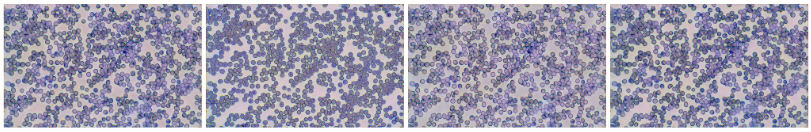
\includegraphics[width=14cm]{gansPics/outputs_from_single_mask.png}
    \caption{Outputs de uma mesma máscara. Fonte: Oleksandr, B; Ham, D; e Noul, Y.}
    \label{fig:fig6}
\end{figure}
\FloatBarrier

Os autores concluem ainda que a geração das imagens é viável para aumentar o volume de dados de um conjunto, desde que não ocorra em um contexto em tempo real. Isso porque o tempo necessário para gerar uma máscara é alto (em média 60 segundos). Gerar a imagem foto-realista, por outro lado, demora 0.5 segundos em média, com uso de GPU.

Para a tarefa de segmentação foi utilizado o modelo FCN-8s, com a função loss sendo (1 - coeficiente de dice), este coeficiente também é utilizado para avaliar os resultados, o treinamento ocorre até que nenhuma melhoria seja observada no modelo.

Os resultados apresentados na figura 7, comparam o modelo treinado com dados reais (RD), dados sintéticos (SD), dados reais augmentados e a combinação destes 3, os métodos de dados augmentados incluem virar imagem horizontalmente e verticalmente, desfoque gaussiano, nitidez, relevo, ruído gaussiano, inversão do canal de cor, mudança de brilho (adição e multiplicação), normalização de contraste e aumento da escala de cinza aplicado aleatoriamente. Todos os modelos foram treinados com 960 imagens e testados com as mesmas 40 imagens reais.
Os experimentos de segmentação demonstraram que os dados sintéticos só melhoram os resultados quando utilizados juntamente com dados reais e dados de augmentação, em outras configurações obtêm resultados ruins, segundos os autores conclusões semelhantes foram observadas em outros estudos na literatura.

Para a tarefa de detecção, foi utilizado o modelo {\it Fast} R-CNN, que precisa de uma grande quantidade de instâncias para treinamento. Assim sendo, utilizar apenas os limitados dados reais disponíveis resultou em uma baixa acurácia (0.781). Por outro lado, quando o modelo é treinado utilizando exclusivamente dados sintéticos, a acurácia aumenta para 0.852. De acordo com os autores, mesmo que seja contra-intuitivo que a acurácia aumente quando utiliza-se apenas dados sintéticos para treino, esse comportamento pode ser explicado pelo fato de se gerar uma variedade maior de formatos e posições de células a partir do gerador de máscaras, do que a variedade disponível no pequeno conjunto de dados reais.

Diferentemente do da Segmentação, o modelo de Detecção de células teve uma melhora de desempenho significativa. Adicionados os dados sintéticos e os dados augmentados aos dados reais, o modelo consegue alcançar uma acurácia de até 0.993, o que representa uma melhora de 27\% da acurácia do modelo.

Devido ao custo computacional de se utilizar R-CNN, os autores propõem uma abordagem que modifica o modelo de segmentação para conter a predição de objetos e contornos dos glóbulos, modifica o modelo de segmentação para funcionar com a predição de objetos e contornos dos glóbulos, e, para a detecção, utiliza um algoritmo simples para identificar bolhas/círculos em imagens binárias. O modelo é mais rápido, porém os resultados são piores em todos os casos. Os autores acreditam que podem melhorar o resultado de segmentação utilizando um modelo mais recente, pois o resultado da detecção depende diretamente dos resultados de segmentação.

\FloatBarrier
\begin{figure}[h]
    \centering
    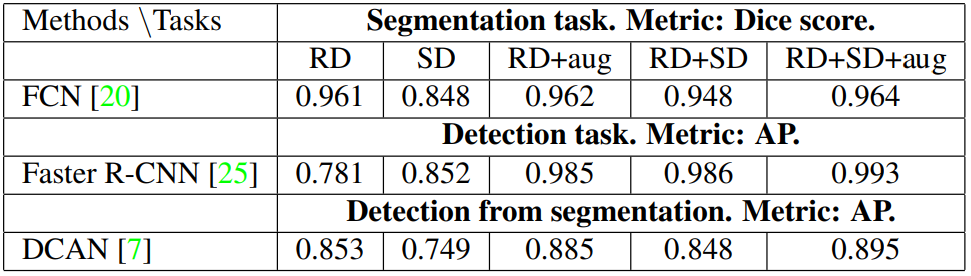
\includegraphics[width=14cm]{gansPics/resultados.png}
    \caption{Avaliação quantitativa em várias tarefas. Fonte: Oleksandr, B; Ham, D; e Noul, Y.}
    \label{fig:fig7}
\end{figure}
\FloatBarrier

Por fim, os autores concluem que a utilização de GANs para {\it augmentar} e gerar dados sintéticos é benéfico para os modelos como foram testados. Entretanto, o ganho de performance pode não compensar o custo de se desenvolver a rede utilizada, como é o caso da tarefa de segmentação (ver figura 7). Os autores também mencionam que o {\it framework} implementado trabalha apenas com glóbulos vermelhos e sugerem que, futuramente, poderão ser implementadas especificações para que o mesmo possa trabalhar com lâminas que, também, apresentem glóbulos brancos e plaquetas.


\printbibliography  \iffalse Mostra as referências em mybib.bib. \fi

\end{document}
